
%% bare_conf.tex
%% V1.3
%% 2007/01/11
%% by Michael Shell
%% See:
%% http://www.michaelshell.org/
%% for current contact information.
%%
%% This is a skeleton file demonstrating the use of IEEEtran.cls
%% (requires IEEEtran.cls version 1.7 or later) with an IEEE conference paper.
%%
%% Support sites:
%% http://www.michaelshell.org/tex/ieeetran/
%% http://www.ctan.org/tex-archive/macros/latex/contrib/IEEEtran/
%% and
%% http://www.ieee.org/

%%*************************************************************************
%% Legal Notice:
%% This code is offered as-is without any warranty either expressed or
%% implied; without even the implied warranty of MERCHANTABILITY or
%% FITNESS FOR A PARTICULAR PURPOSE! 
%% User assumes all risk.
%% In no event shall IEEE or any contributor to this code be liable for
%% any damages or losses, including, but not limited to, incidental,
%% consequential, or any other damages, resulting from the use or misuse
%% of any information contained here.
%%
%% All comments are the opinions of their respective authors and are not
%% necessarily endorsed by the IEEE.
%%
%% This work is distributed under the LaTeX Project Public License (LPPL)
%% ( http://www.latex-project.org/ ) version 1.3, and may be freely used,
%% distributed and modified. A copy of the LPPL, version 1.3, is included
%% in the base LaTeX documentation of all distributions of LaTeX released
%% 2003/12/01 or later.
%% Retain all contribution notices and credits.
%% ** Modified files should be clearly indicated as such, including  **
%% ** renaming them and changing author support contact information. **
%%
%% File list of work: IEEEtran.cls, IEEEtran_HOWTO.pdf, bare_adv.tex,
%%                    bare_conf.tex, bare_jrnl.tex, bare_jrnl_compsoc.tex
%%*************************************************************************

% *** Authors should verify (and, if needed, correct) their LaTeX system  ***
% *** with the testflow diagnostic prior to trusting their LaTeX platform ***
% *** with production work. IEEE's font choices can trigger bugs that do  ***
% *** not appear when using other class files.                            ***
% The testflow support page is at:
% http://www.michaelshell.org/tex/testflow/



% Note that the a4paper option is mainly intended so that authors in
% countries using A4 can easily print to A4 and see how their papers will
% look in print - the typesetting of the document will not typically be
% affected with changes in paper size (but the bottom and side margins will).
% Use the testflow package mentioned above to verify correct handling of
% both paper sizes by the user's LaTeX system.
%
% Also note that the "draftcls" or "draftclsnofoot", not "draft", option
% should be used if it is desired that the figures are to be displayed in
% draft mode.
%
\documentclass[conference]{IEEEtran}
\usepackage{graphicx, amsmath, algorithm, tikz, algpseudocode}%, algorithmic}
% Add the compsoc option for Computer Society conferences.
%
% If IEEEtran.cls has not been installed into the LaTeX system files,
% manually specify the path to it like:
% \documentclass[conference]{../sty/IEEEtran}





% Some very useful LaTeX packages include:
% (uncomment the ones you want to load)


% *** MISC UTILITY PACKAGES ***
%
%\usepackage{ifpdf}
% Heiko Oberdiek's ifpdf.sty is very useful if you need conditional
% compilation based on whether the output is pdf or dvi.
% usage:
% \ifpdf
%   % pdf code
% \else
%   % dvi code
% \fi
% The latest version of ifpdf.sty can be obtained from:
% http://www.ctan.org/tex-archive/macros/latex/contrib/oberdiek/
% Also, note that IEEEtran.cls V1.7 and later provides a builtin
% \ifCLASSINFOpdf conditional that works the same way.
% When switching from latex to pdflatex and vice-versa, the compiler may
% have to be run twice to clear warning/error messages.






% *** CITATION PACKAGES ***
%
%\usepackage{cite}
% cite.sty was written by Donald Arseneau
% V1.6 and later of IEEEtran pre-defines the format of the cite.sty package
% \cite{} output to follow that of IEEE. Loading the cite package will
% result in citation numbers being automatically sorted and properly
% "compressed/ranged". e.g., [1], [9], [2], [7], [5], [6] without using
% cite.sty will become [1], [2], [5]--[7], [9] using cite.sty. cite.sty's
% \cite will automatically add leading space, if needed. Use cite.sty's
% noadjust option (cite.sty V3.8 and later) if you want to turn this off.
% cite.sty is already installed on most LaTeX systems. Be sure and use
% version 4.0 (2003-05-27) and later if using hyperref.sty. cite.sty does
% not currently provide for hyperlinked citations.
% The latest version can be obtained at:
% http://www.ctan.org/tex-archive/macros/latex/contrib/cite/
% The documentation is contained in the cite.sty file itself.


\usepackage[utf8]{inputenc}



% *** GRAPHICS RELATED PACKAGES ***
%
\ifCLASSINFOpdf
  % \usepackage[pdftex]{graphicx}
  % declare the path(s) where your graphic files are
  % \graphicspath{{../pdf/}{../jpeg/}}
  % and their extensions so you won't have to specify these with
  % every instance of \includegraphics
  % \DeclareGraphicsExtensions{.pdf,.jpeg,.png}
\else
  % or other class option (dvipsone, dvipdf, if not using dvips). graphicx
  % will default to the driver specified in the system graphics.cfg if no
  % driver is specified.
  % \usepackage[dvips]{graphicx}
  % declare the path(s) where your graphic files are
  % \graphicspath{{../eps/}}
  % and their extensions so you won't have to specify these with
  % every instance of \includegraphics
  % \DeclareGraphicsExtensions{.eps}
\fi
% graphicx was written by David Carlisle and Sebastian Rahtz. It is
% required if you want graphics, photos, etc. graphicx.sty is already
% installed on most LaTeX systems. The latest version and documentation can
% be obtained at: 
% http://www.ctan.org/tex-archive/macros/latex/required/graphics/
% Another good source of documentation is "Using Imported Graphics in
% LaTeX2e" by Keith Reckdahl which can be found as epslatex.ps or
% epslatex.pdf at: http://www.ctan.org/tex-archive/info/
%
% latex, and pdflatex in dvi mode, support graphics in encapsulated
% postscript (.eps) format. pdflatex in pdf mode supports graphics
% in .pdf, .jpeg, .png and .mps (metapost) formats. Users should ensure
% that all non-photo figures use a vector format (.eps, .pdf, .mps) and
% not a bitmapped formats (.jpeg, .png). IEEE frowns on bitmapped formats
% which can result in "jaggedy"/blurry rendering of lines and letters as
% well as large increases in file sizes.
%
% You can find documentation about the pdfTeX application at:
% http://www.tug.org/applications/pdftex





% *** MATH PACKAGES ***
%
%\usepackage[cmex10]{amsmath}
% A popular package from the American Mathematical Society that provides
% many useful and powerful commands for dealing with mathematics. If using
% it, be sure to load this package with the cmex10 option to ensure that
% only type 1 fonts will utilized at all point sizes. Without this option,
% it is possible that some math symbols, particularly those within
% footnotes, will be rendered in bitmap form which will result in a
% document that can not be IEEE Xplore compliant!
%
% Also, note that the amsmath package sets \interdisplaylinepenalty to 10000
% thus preventing page breaks from occurring within multiline equations. Use:
%\interdisplaylinepenalty=2500
% after loading amsmath to restore such page breaks as IEEEtran.cls normally
% does. amsmath.sty is already installed on most LaTeX systems. The latest
% version and documentation can be obtained at:
% http://www.ctan.org/tex-archive/macros/latex/required/amslatex/math/





% *** SPECIALIZED LIST PACKAGES ***
%
%\usepackage{algorithmic}
% algorithmic.sty was written by Peter Williams and Rogerio Brito.
% This package provides an algorithmic environment fo describing algorithms.
% You can use the algorithmic environment in-text or within a figure
% environment to provide for a floating algorithm. Do NOT use the algorithm
% floating environment provided by algorithm.sty (by the same authors) or
% algorithm2e.sty (by Christophe Fiorio) as IEEE does not use dedicated
% algorithm float types and packages that provide these will not provide
% correct IEEE style captions. The latest version and documentation of
% algorithmic.sty can be obtained at:
% http://www.ctan.org/tex-archive/macros/latex/contrib/algorithms/
% There is also a support site at:
% http://algorithms.berlios.de/index.html
% Also of interest may be the (relatively newer and more customizable)
% algorithmicx.sty package by Szasz Janos:
% http://www.ctan.org/tex-archive/macros/latex/contrib/algorithmicx/




% *** ALIGNMENT PACKAGES ***
%
%\usepackage{array}
% Frank Mittelbach's and David Carlisle's array.sty patches and improves
% the standard LaTeX2e array and tabular environments to provide better
% appearance and additional user controls. As the default LaTeX2e table
% generation code is lacking to the point of almost being broken with
% respect to the quality of the end results, all users are strongly
% advised to use an enhanced (at the very least that provided by array.sty)
% set of table tools. array.sty is already installed on most systems. The
% latest version and documentation can be obtained at:
% http://www.ctan.org/tex-archive/macros/latex/required/tools/


%\usepackage{mdwmath}
%\usepackage{mdwtab}
% Also highly recommended is Mark Wooding's extremely powerful MDW tools,
% especially mdwmath.sty and mdwtab.sty which are used to format equations
% and tables, respectively. The MDWtools set is already installed on most
% LaTeX systems. The lastest version and documentation is available at:
% http://www.ctan.org/tex-archive/macros/latex/contrib/mdwtools/


% IEEEtran contains the IEEEeqnarray family of commands that can be used to
% generate multiline equations as well as matrices, tables, etc., of high
% quality.


%\usepackage{eqparbox}
% Also of notable interest is Scott Pakin's eqparbox package for creating
% (automatically sized) equal width boxes - aka "natural width parboxes".
% Available at:
% http://www.ctan.org/tex-archive/macros/latex/contrib/eqparbox/





% *** SUBFIGURE PACKAGES ***
%\usepackage[tight,footnotesize]{subfigure}
% subfigure.sty was written by Steven Douglas Cochran. This package makes it
% easy to put subfigures in your figures. e.g., "Figure 1a and 1b". For IEEE
% work, it is a good idea to load it with the tight package option to reduce
% the amount of white space around the subfigures. subfigure.sty is already
% installed on most LaTeX systems. The latest version and documentation can
% be obtained at:
% http://www.ctan.org/tex-archive/obsolete/macros/latex/contrib/subfigure/
% subfigure.sty has been superceeded by subfig.sty.



%\usepackage[caption=false]{caption}
%\usepackage[font=footnotesize]{subfig}
% subfig.sty, also written by Steven Douglas Cochran, is the modern
% replacement for subfigure.sty. However, subfig.sty requires and
% automatically loads Axel Sommerfeldt's caption.sty which will override
% IEEEtran.cls handling of captions and this will result in nonIEEE style
% figure/table captions. To prevent this problem, be sure and preload
% caption.sty with its "caption=false" package option. This is will preserve
% IEEEtran.cls handing of captions. Version 1.3 (2005/06/28) and later 
% (recommended due to many improvements over 1.2) of subfig.sty supports
% the caption=false option directly:
%\usepackage[caption=false,font=footnotesize]{subfig}
%
% The latest version and documentation can be obtained at:
% http://www.ctan.org/tex-archive/macros/latex/contrib/subfig/
% The latest version and documentation of caption.sty can be obtained at:
% http://www.ctan.org/tex-archive/macros/latex/contrib/caption/




% *** FLOAT PACKAGES ***
%
%\usepackage{fixltx2e}
% fixltx2e, the successor to the earlier fix2col.sty, was written by
% Frank Mittelbach and David Carlisle. This package corrects a few problems
% in the LaTeX2e kernel, the most notable of which is that in current
% LaTeX2e releases, the ordering of single and double column floats is not
% guaranteed to be preserved. Thus, an unpatched LaTeX2e can allow a
% single column figure to be placed prior to an earlier double column
% figure. The latest version and documentation can be found at:
% http://www.ctan.org/tex-archive/macros/latex/base/



%\usepackage{stfloats}
% stfloats.sty was written by Sigitas Tolusis. This package gives LaTeX2e
% the ability to do double column floats at the bottom of the page as well
% as the top. (e.g., "\begin{figure*}[!b]" is not normally possible in
% LaTeX2e). It also provides a command:
%\fnbelowfloat
% to enable the placement of footnotes below bottom floats (the standard
% LaTeX2e kernel puts them above bottom floats). This is an invasive package
% which rewrites many portions of the LaTeX2e float routines. It may not work
% with other packages that modify the LaTeX2e float routines. The latest
% version and documentation can be obtained at:
% http://www.ctan.org/tex-archive/macros/latex/contrib/sttools/
% Documentation is contained in the stfloats.sty comments as well as in the
% presfull.pdf file. Do not use the stfloats baselinefloat ability as IEEE
% does not allow \baselineskip to stretch. Authors submitting work to the
% IEEE should note that IEEE rarely uses double column equations and
% that authors should try to avoid such use. Do not be tempted to use the
% cuted.sty or midfloat.sty packages (also by Sigitas Tolusis) as IEEE does
% not format its papers in such ways.





% *** PDF, URL AND HYPERLINK PACKAGES ***
%
%\usepackage{url}
% url.sty was written by Donald Arseneau. It provides better support for
% handling and breaking URLs. url.sty is already installed on most LaTeX
% systems. The latest version can be obtained at:
% http://www.ctan.org/tex-archive/macros/latex/contrib/misc/
% Read the url.sty source comments for usage information. Basically,
% \url{my_url_here}.





% *** Do not adjust lengths that control margins, column widths, etc. ***
% *** Do not use packages that alter fonts (such as pslatex).         ***
% There should be no need to do such things with IEEEtran.cls V1.6 and later.
% (Unless specifically asked to do so by the journal or conference you plan
% to submit to, of course. )


% correct bad hyphenation here
%\hyphenation{op-tical net-works semi-conduc-tor}


\begin{document}
%
% paper title
% can use linebreaks \\ within to get better formatting as desired
\title{Wildfire Spreading Model using a Parallel Implementation of Cellular Automata}
%\title{Designing a Simulator for Wildfire Spreading based in Cellular Automata} 
%\title{A Wildfire Model based in Cellular Automata }


%author names and affiliations
%use a multiple column layout for up to three different
%affiliations
% \author{\IEEEauthorblockN{Michael Shell}
% \IEEEauthorblockA{School of Electrical and\\Computer Engineering\\
% Georgia Institute of Technology\\
% Atlanta, Georgia 30332--0250\\
% Email: http://www.michaelshell.org/contact.html}
% \and
% \IEEEauthorblockN{Homer Simpson}
% \IEEEauthorblockA{Twentieth Century Fox\\
% Springfield, USA\\
% Email: homer@thesimpsons.com}
% \and
% \IEEEauthorblockN{James Kirk\\ and Montgomery Scott}
% \IEEEauthorblockA{Starfleet Academy\\
% San Francisco, California 96678-2391\\
% Telephone: (800) 555--1212\\
% Fax: (888) 555--1212}}

\author{
    \IEEEauthorblockN{Roberto G. Aldunate}
    \IEEEauthorblockA{College of Applied Health Sciences\\
    University of Illinois at Urbana–Champaign, \\ Champaign, USA\\ aldunate@illinois.edu}
    \and
    \IEEEauthorblockN{Daniel San Martín}
    \IEEEauthorblockA{Departamento de Informática\\
    Universidad Técnica Federico Santa María, \\ Valparaíso, Chile\\ daniel.sanmartinr@sansano.usm.cl}
}

% \author{\IEEEauthorblockN{Michael Shell}
% \IEEEauthorblockA{School of Electrical and\\Computer Engineering\\
% Georgia Institute of Technology\\
% Atlanta, Georgia 30332--0250\\
% Email: http://www.michaelshell.org/contact.html}
% \and
% \IEEEauthorblockN{Homer Simpson}
% \IEEEauthorblockA{Twentieth Century Fox\\
% Springfield, USA\\
% Email: homer@thesimpsons.com}

% conference papers do not typically use \thanks and this command
% is locked out in conference mode. If really needed, such as for
% the acknowledgment of grants, issue a \IEEEoverridecommandlockouts
% after \documentclass

% for over three affiliations, or if they all won't fit within the width
% of the page, use this alternative format:
% 
%\author{\IEEEauthorblockN{Michael Shell\IEEEauthorrefmark{1},
%Homer Simpson\IEEEauthorrefmark{2},
%James Kirk\IEEEauthorrefmark{3}, 
%Montgomery Scott\IEEEauthorrefmark{3} and
%Eldon Tyrell\IEEEauthorrefmark{4}}
%\IEEEauthorblockA{\IEEEauthorrefmark{1}School of Electrical and Computer Engineering\\
%Georgia Institute of Technology,
%Atlanta, Georgia 30332--0250\\ Email: see http://www.michaelshell.org/contact.html}
%\IEEEauthorblockA{\IEEEauthorrefmark{2}Twentieth Century Fox, Springfield, USA\\
%Email: homer@thesimpsons.com}
%\IEEEauthorblockA{\IEEEauthorrefmark{3}Starfleet Academy, San Francisco, California 96678-2391\\
%Telephone: (800) 555--1212, Fax: (888) 555--1212}
%\IEEEauthorblockA{\IEEEauthorrefmark{4}Tyrell Inc., 123 Replicant Street, Los Angeles, California 90210--4321}}




% use for special paper notices
%\IEEEspecialpapernotice{(Invited Paper)}




% make the title area
\maketitle


\begin{abstract}
%\boldmath
%\blindtext[1]
    Wildfires may have devastating social and economic impact in our societies, destroying thousands of 
    forest hectares that also dramatically damage the ecosystems. There is a pressing need to better understand, 
    framed in disaster response decision making, and control wildfires in different geographical areas. There 
    are continuous and discrete mathematical models that aim to explain and model wildfire’s dynamics, but is 
    necessary to integrate a wildfire model into a larger container that enables first responders to simulate 
    and rehearse responses to wildfire propagation dynamics. This work presents a Cellular Automata-based 
    model incorporated into a simulator built for the Chilean forest protection agency (CONAF), which is implemented 
    as a service for a video game-based simulator. Results include very encouraging evaluation from the Chilean 
    forest agency, while conclusions highlight that video game technology is extremely appropriate to implement 
    and evaluate wildfire’s dynamics on varying environments.
\end{abstract}
% IEEEtran.cls defaults to using nonbold math in the Abstract.
% This preserves the distinction between vectors and scalars. However,
% if the journal you are submitting to favors bold math in the abstract,
% then you can use LaTeX's standard command \boldmath at the very start
% of the abstract to achieve this. Many IEEE journals frown on math
% in the abstract anyway.

% Note that keywords are not normally used for peerreview papers.
\begin{IEEEkeywords}
    Wildfire, Cellular Automata, Parallel Programming.
\end{IEEEkeywords}

% For peer review papers, you can put extra information on the cover
% page as needed:
% \ifCLASSOPTIONpeerreview
% \begin{center} \bfseries EDICS Category: 3-BBND \end{center}
% \fi
%
% For peerreview papers, this IEEEtran command inserts a page break and
% creates the second title. It will be ignored for other modes.
\IEEEpeerreviewmaketitle



\section{Introduction}
    % The Fire Spreading is one of the most harmful phenomena in Chile, burning thousands of forest hectares, 
    % destroying the flora and fauna, affecting the air, the water cycles and the ecosystem present in this places. 
    % These damages generate economics, environmental and social losses that are fighting by 2 protection systems, 
    % one made up of the private sector and the other by the state. The fire origin may be related to the people 
    % neglect with the use of heat sources over fuel vegetation, poor environment culture and even in deliberately way.
    % Nevertheless, this is not only the fire spreading causes, the fire also started under some environment conditions 
    % as extreme temperatures, drought periods, and strong winds, among others and mean about 5000 and 7000 forest fires. 
    % In surface terms, the damage averages about 52000 hectares burnt and in extreme periods have ranged from 10000 
    % and 101000 hectares \cite{fireCONAF}.
    % Wildfires are one of the most harmful phenomena in Chile burning thousands of forest hectares every year, 
    % destroying significant flora and fauna, while affecting the air, water cycles, and the ecosystem. Origins of 
    % wildfires are due to several reasons, ranging from reckless people starting fires without care for the environment, 
    % to behaving in a deliberately way, to extreme weather and environmental conditions. Yearly, burnt hectares are in
    % the order of 50,000, but in certain occasions up to 100,000 have been consumed by fire \cite{fireCONAF}. \\
    
    % Wildfire spreading dynamics has gathered large attention form the scientific community. In general, modeling 
    % wildfire is accomplished by using continuous or discrete models, or a combination of both \cite{muzy2005modelling,
    % ferragut2007modelling,brun2013coupling, bianchini2015evolutionary}.
    % Continuous modeling attempts to represent the fire dynamics using mostly differential equations 
    % \cite{morvan2001modeling,asensio2005convection,ferragut2007numerical,glasa2008elliptical,morvan2009physical,
    % silvani2009fire,denham2012dynamic,eberle2014forest,eberle2014modeling,gorham2014studying,ferragut2015wildland,
    % morales2015stochastic,bufacchi2016numerical,el2016experimental}. 
    % On the other hand, wildfire discrete modeling is characterized by the use of discrete simulation techniques such as 
    % Cellular Automata \cite{karafyllidis1997model,muzy2005specification,ntaimo2006two,muzy2006dynamic,alexandridis2008cellular,
    % muzy2008discrete,filippi2010discrete,hu2012devs,wainer2016modelling,fernandez2017two}. \\
    
    % Literature review shows that there is a large percentage of research efforts that use continuous models for 
    % wildfire modeling, the research presented in this article uses discrete modeling mainly because of the possibility 
    % to easily incorporate lower level details about geographically dependent features, such as flora, water areas, and 
    % location-based responses or fire combat. This research effort is part of a research project titled ``Serious video 
    % games to improve decision making for disaster response systems'' (FONDEF-CA13I10331) (31) funded by the Chilean 
    % national science foundation, and as such the CA modeling effort fit seamlessly with teach one of the three high 
    % priority forest reserves used in this project. \\
    
    % While the core of any wildfire propagation model is well understood and there are plenty of options from where to 
    % take ideas when building another simulator, e.g., Australian simulator developed by the National Bushfire Research 
    % Unit (32) or Chile-an simulator developed by Universidad de Chile; KITRAL (33), (34) defining inputs such as terrain 
    % characteristics, fuel type, meteorological conditions, and fire characteristics, statistical past patterns, among 
    % others, the dynamic interplay between variables such as temperature, humidity, pressure, and wind characteristics 
    % are an elusive component for most of wildfire modeling efforts. The project framing this article aims to incorporate 
    % dynamic changes on temperature, humidity, pressure, and wind characteristics, but in a later stage. Nevertheless, the 
    % framework for this modeling effort is included in this article. \\

    % The goal for this research initiative is to build an appropriate model to be incorporated into a video game–based 
    % simulator, a Unity3D engine based platform, to al-low assessment of decision making during wildfire combat involving 
    % different agencies which are part of the response system; National Forest Corporation (CONAF) 
    % and National Emergencies Office (ONEMI). For this goal, three high priority protected areas 
    % defined by CONAF from the Valparaiso Region in Chile where modeled so that these video game scenarios may: a) be expanded
    % later with dynamic interplay between temperature, pressure, humidity, and wind characteristics; and b) be easily used 
    % as models to generate corresponding scenarios for other regions in the country, or any other geo-graphical location. \\
    
    % The remaining of this article is structure as follows; next section presents the design of the model proposed in this 
    % research initiative. The section after that shows the implementation of the model, followed by a section describing 
    % the results obtained when incorporated the implemented model into the Unity3D-based platform and the evaluation from 
    % Chilean national forest protection agency. Finally, discussion and conclusions are presented.
    
    Wildfires are one of the most harmful phenomena in Chile burning thousands of forest hectares every year 
    destroying significant flora and fauna, and affecting the air, water cycles, and the ecosystem. Wildfires 
    start by varied reasons, ranging from reckless human behavior to extreme weather and environmental conditions. 
    In Chile, around 50000 hectares are burnt yearly, and in certain occasions up to 100000 hectares have 
    been consumed by fire \cite{fireCONAF}.

    Wildfire spreading dynamics has gathered large attention from the scientific community. In general, 
    wildfires are modelled using continuous or discrete models, or a combination of both \cite{brun2013coupling, 
    bianchini2015evolutionary}. Many authors use differential equations for continuous modelling 
    \cite{rothermel1972mathematical,ferragut2015wildland,bufacchi2016numerical,el2016experimental}, but 
    discrete modelling has also gained significant interest from the scientific community; specially the use 
    Cellular Automata \cite{karafyllidis1997model,alexandridis2008cellular,wainer2016modelling,fernandez2017two}, 
    to model wildfire dynamics. 
    
    This research effort is part of a research project titled ``Serious video games to improve decision making for 
    disaster response systems'' \cite{aldunate} funded by Chile’s national science foundation. The research presented in this 
    article uses discrete modeling because of the possibility to easily incorporate lower level details about 
    geographically dependent features, such as flora, water areas, and location-based responses or fire combat, 
    and fine granularity to incorporate dynamic interplay among temperature, humidity, and wind characteristics.
    While there is significant consensus on modelling core components of wildfire propagation models, such as 
    terrain characteristics, fuel type, meteorological conditions, statistical past patterns, the dynamic interaction 
    between temperature, humidity, pressure, and wind characteristics are usually an elusive component in most modelling efforts. 
    
    The goal for this research initiative is to build a suitable model to be incorporated into a video-game-based 
    simulator to allow assessment of decision making during wildfire combat involving different agencies which are 
    part of the response system in Chile; the National Forest Agency (CONAF) and the National Emergencies Agency. 
    For this goal, instead of developing complex continuous or discrete models that may forecast and reproduce 
    wildfire dynamics in a realistic manner based only on mathematical models, this work proposes the use of a 
    hybrid approach, which provides mathematical models for core capability of wildfire propagation dynamics, 
    but also incorporates the expert role who may qualitatively alter the model dynamics in real-time to generate 
    realistic cases for further use in the video-game-based simulator. The expert executes actions in the wildfire 
    propagation dynamics through parameters such as wind speed and direction, temperature, and humidity as well as 
    through changes in transition functions in the cellular automata.

%\subsection{Subsection Heading Here}
%\blindtext

% needed in second column of first page if using \IEEEpubid
%\IEEEpubidadjcol

% An example of a floating figure using the graphicx package.
% Note that \label must occur AFTER (or within) \caption.
% For figures, \caption should occur after the \includegraphics.
% Note that IEEEtran v1.7 and later has special internal code that
% is designed to preserve the operation of \label within \caption
% even when the captionsoff option is in effect. However, because
% of issues like this, it may be the safest practice to put all your
% \label just after \caption rather than within \caption{}.
%
% Reminder: the "draftcls" or "draftclsnofoot", not "draft", class
% option should be used if it is desired that the figures are to be
% displayed while in draft mode.
%
%\begin{figure}[!t]
%\centering
%\includegraphics[width=2.5in]{myfigure}
% where an .eps filename suffix will be assumed under latex, 
% and a .pdf suffix will be assumed for pdflatex; or what has been declared
% via \DeclareGraphicsExtensions.
%\caption{Simulation Results}
%\label{fig_sim}
%\end{figure}

% Note that IEEE typically puts floats only at the top, even when this
% results in a large percentage of a column being occupied by floats.


% An example of a double column floating figure using two subfigures.
% (The subfig.sty package must be loaded for this to work.)
% The subfigure \label commands are set within each subfloat command, the
% \label for the overall figure must come after \caption.
% \hfil must be used as a separator to get equal spacing.
% The subfigure.sty package works much the same way, except \subfigure is
% used instead of \subfloat.
%
%\begin{figure*}[!t]
%\centerline{\subfloat[Case I]\includegraphics[width=2.5in]{subfigcase1}%
%\label{fig_first_case}}
%\hfil
%\subfloat[Case II]{\includegraphics[width=2.5in]{subfigcase2}%
%\label{fig_second_case}}}
%\caption{Simulation results}
%\label{fig_sim}
%\end{figure*}
%
% Note that often IEEE papers with subfigures do not employ subfigure
% captions (using the optional argument to \subfloat), but instead will
% reference/describe all of them (a), (b), etc., within the main caption.


% An example of a floating table. Note that, for IEEE style tables, the 
% \caption command should come BEFORE the table. Table text will default to
% \footnotesize as IEEE normally uses this smaller font for tables.
% The \label must come after \caption as always.
%
%\begin{table}[!t]
%% increase table row spacing, adjust to taste
%\renewcommand{\arraystretch}{1.3}
% if using array.sty, it might be a good idea to tweak the value of
% \extrarowheight as needed to properly center the text within the cells
%\caption{An Example of a Table}
%\label{table_example}
%\centering
%% Some packages, such as MDW tools, offer better commands for making tables
%% than the plain LaTeX2e tabular which is used here.
%\begin{tabular}{|c||c|}
%\hline
%One & Two\\
%\hline
%Three & Four\\
%\hline
%\end{tabular}
%\end{table}


% Note that IEEE does not put floats in the very first column - or typically
% anywhere on the first page for that matter. Also, in-text middle ("here")
% positioning is not used. Most IEEE journals use top floats exclusively.
% Note that, LaTeX2e, unlike IEEE journals, places footnotes above bottom
% floats. This can be corrected via the \fnbelowfloat command of the
% stfloats package.

\section{Formalization}
    
    %The aim of this work is to develop a tool capable to give the possibilty of tr
    %Given the nature of this phenomenon, it is necessary to have tools that support the study and control of fire. 
    %This work aims to develop a tool that
    %Since the nature of this phenomena, it becomes necessary to build tools for the 
    %Since we have to integrate all the mathematical and computational components to build a useful simulator
    %system, it becomes necessary to maximize the computational resources because the dynamic system and
    %video-game-based tool consumes 
    
    The problem presented in this paper is related to the complexity of incorporating a hybrid 
    approach in the development of the simulator, which allows qualitatively modeling the wildfire
    and also adds the dynamic component in which the expert role makes changes in real time.
    
    Due to the objective of the model is to be as realistic as possible, the model must handle a 
    high resolution of the terrain to be modeled, involving the management of high dimension matrices 
    consecutively.
    
    Within the motivations of the development of this simulator there is the possibility of 
    training the technical and professional personnel involved in the combat of this type of 
    disaster. It is clear that proposing a realistic experience allows a positive impact on the 
    decision-making processes and complements in an important way the classical techniques of 
    teaching and training in this area.

    

\section{Solution}

    For the development of the simulator, the fire model was constructed using 
    environmental factors, forest fuel, topography and the cellular automata which interact and evolve in 
    discrete time steps. Then, to include the dynamic component, it was necessary to enhance 
    the computation of the model with parallel computing techniques. The elements involves in the
    development of the simulator are described in detail below.

    %The main components used for our wildfire model are environmental factors, forest fuel,
    %topography and the cellular automata. These elements are described in detail below.
    
    
    \subsection{Environmental factors}
        
        The environmental factors are closely related with the fire propagation. The wind guides the fire’s direction, 
        brings oxygen, and increases the speed of fire propagation, dried fuel and transports sparks. Temperature evaporates
        the humidity from fuels, increasing the chances of to burn. If the relative humidity is low, the fuel is drier than 
        the reverse case, it is therefore more flammable. There is not vertical movement of air masses when the atmospheric is
        quiet, on the contrary with atmospheric instability there are strong wind current stimulating the fire spreading. \\
        
        Since we work in a discrete world, the environmental factors were discretized (values between $0$ and $1$) using the 
        typical weather values in Chile. We can summarize the relations between the fire and environmental factors as: the 
        temperature and wind have a direct and the humidity and pressure have an inversely effect to the fire spread speed. 

    
    \subsection{Forest Fuel}
    
        The forest fuel are all the vegetation elements, woody or herbaceous, alive or dead
        that may be flammable. These elements are classified by: type, location, size, amount,
        humidity, compression, continuity, and chemical content. A simple scalar
        is used in the model to moderate the impact of this component of the probability for each cell of
        the cellular automata to start and stop burning.
        
        
    \subsection{Topography}
    
        The topography factor influences over the two above factors, the fuel and weather,
        modifying or altering them. The fire dynamics may be affected by: (a) the slope; it
        favors the rise of convection currents of warm air preheating fuels above, accelerating
        the wildfire; (b) altitude: at higher altitudes, the temperature is cooler; there is greater
        precipitation and snow reducing the amount of oxygen in the air; (c) exposure: affects
        the behavior of wind and hot sun; (d) landform: affects wind patterns and temperature
        in a given locality. At the present version of the model, this set of factors are modeled
        with a single scalar that may reduce or magnify the chances for cells to start / stop
        burning. Further versions of this work will include more elaborate versions of sub
        models that will embrace the articulation of the topography factors. \\
        
        In addition, according to CONAF, there are 3 models for wildfire progression: (a)
        circular: in this case, the terrain is flat, there is no wind presence and the fuel is
        uniform; (b) oval: In this case, the land has a smooth slope, there is soft wind and the
        fuel is heterogeneous; and (c) extended: The terrain is sloped, exist strong wind and
        the fuel is heterogeneous. Most of the scenarios involved in this work were flat, the
        type of wildfire progression was considered circular, in absence of wind and other
        factors. Further work will include the impact of this element for scenarios that exhibit
        these three types of wildfire progression.
    

    \subsection{Cellular Automata}
    
        John Von Neumann introduced the Cellular Automata (CA) in 1966, this appears as an alternative option to 
        models that use partial differential equations (PDE) and satisfactory results have demonstrated in physics 
        models \cite{toffoli1984cellular}. CA have been used to model complex systems \cite{wolfram1994cellular} 
        and applied to some physics problems where local iterations are involved \cite{chopard1991cellular, 
        gerhardt1989cellular}. The discrete nature of CA allows plenty of opportunity to include elements at local 
        level that have the potential to achieve a suitable emerging solution for wildfire dynamics modeling. 
        The main characteristics of the CA used in this work are as follows:
        
        \subsubsection{Spatial dimensions}
        
            The number of spatial dimensions gives the sense of simulation space. In this model, the simulation has 
            two spatial dimensions, that is, the CA has cells in $(i,j)$ in a grid of size $M\times N$.
            
        \subsubsection{Neighborhood}
        
            This CA model use the Moore Neighborhood \cite{moorewolfram} that is a squared region used 
            to define a set of cells around a cell $(i_0,j_0)$. The Moore neighborhood of range $r$ is defined by
            \begin{equation}
                N_{(i_0,j_0)}^M = \{(i,j): ~ |i-i_0|\leq r, ~ |j-j_0|\leq r \}.
            \end{equation}
            
            The range used in this work was $r=1$.

            %This definition applied to the model with range $r=1$  is represented by Figure 1.
            
        \subsubsection{Cell states}
        
            To represent the fire spreading phenomena applied to the CA theory is necessary to define the cell states. 
            In this work we define: nonflammable = $0$; flammable = $1$; burning = $2$; burnt = $3$; extinguished = $4$.
            
            % \begin{table}[!ht]
            %     \centering
            %     \caption{CA states ($S_{i,i})$}
            %     \begin{tabular}{|c|c|}
            %         \hline
            %         \textbf{State} & \textbf{Value}  \\ \hline
            %         Nonflammable & 0 \\ \hline
            %         Flammable & 1 \\ \hline
            %         Burning & 2 \\ \hline
            %         Burnt & 3 \\ \hline
            %         Extinguished & 4 \\ \hline
            %     \end{tabular}
            %     \label{tab:CAstates}
            % \end{table}
            
        
        \subsubsection{Transition Rule}
        
            The transition rule computes the future value of the respective cells. For this case
            the cell’s next state is computed as: 
            \begin{equation}
                \begin{split}
                    S_{i,j}^{t+1} = F(S_{i,j}^t,S_{i,j+1}^t, S_{i+1,j+1}^t,S_{i+1,j}^t, S_{i+1,j-1}^t, S_{i,j-1}^t, \\ \nonumber
                    S_{i,j-1}^t, S_{i-1,j-1}^t, S_{i-1,j}^t, S_{i-1,j+1}^t, T, H, W_s, W_d, F_{ab})
                \end{split}
                \label{eq:transition_rule}
            \end{equation}
            
            where $T$ is the temperature, $H$ the humidity, $W_s$ the speed and $W_d$ direction of wind, $F_{ab}$ the 
            probability of change from state $a$ to $b$. \\
            
            %To simulate the transition from a state to another the follow rules are proposed:
            Formally, we propose the follow transition rule:
            \begin{equation}
                S_{i,j}^{t+1} =
                \begin{cases}
                    %0, ~ if ~ S_{i,j}^{t} = 0 \\
                    %1, ~ if ~ S_{i,j}^{t} = 1 \\
                    2, & \text{if} ~ S_{i,j}^{t} = 1 ~ \text{and} ~ f_{12} \geq F_{12} \\
                    2, & \text{if} ~ S_{i,j}^{t} = 4 ~ \text{and} ~ f_{42} \leq F_{42} \\
                    3, & \text{if} ~ S_{i,j}^{t} = 2 ~ \text{and} ~ f_{23} \leq F_{23} \\
                    4, & \text{if} ~ S_{i,j}^{t} = 3 ~ \text{and} ~ f_{24} \leq F_{24}
                \end{cases},
            \end{equation}
            
            where the functions $f$ are determined by the following equations:
            
            \begin{itemize}
                \item Function $f_{12}$: represents the probability that a cell begin to burn and depend of:
                    \begin{itemize}
                        \item The environmental factors $E$, described before and represented by:
                            \begin{equation}
                                E = \frac{a \cdot T \cdot W_s}{H \cdot P},
                            \end{equation}
                            where $a$ is a factor that depends of wind direction. This factor is computed by
                            \begin{equation}
                                a = 
                                \begin{cases}
                                    1 & \text{if cell in the same direction} \\
                                     & \text{of $W_d$ is burning.}\\
                                    2/3 & \text{if contiguous cells in the same} \\
                                     & \text{direction of $W_d$ are burning.} \\
                                    1/3 & \text{otherwise.}
                                \end{cases}
                            \end{equation}
                            
                        \item Terrain fuel composition $c$ with $0\leq c\leq 1$.
                        \item The burning states of neighborhood $p(N_b)$ defined by
                            \begin{equation}
                                p(N_b) = \frac{N_b}{8},
                            \end{equation}
                            where $N_b$ is the number of burning state neighboring cells.
                        \end{itemize}
                        Finally, $f_{12}$ is computed by
                            \begin{equation}
                                f_{12} = \alpha \cdot c\cdot E + \beta \cdot p(N_b).
                            \end{equation}
                            
                            $\alpha$ and $\beta$ ($\alpha+\beta = 1$) is used to weight the effect of weather condition 
                            and neighborhood respectively.
                    
                \item Function $f_{23}$: represents the probability that a cell ends up burning and is defined as random value between $0$ and $1$.
                \item Function $f_{24}$: represents the probability that a cell is extinguished and is defined as random value between $0$ and $1$.
                \item Function $f_{42}$: represents the probability that an extinct cell burns again and is defined as random value between $0$ and $1$.
            \end{itemize}
            
            $F_{12}, F_{23}, F_{24}, F_{42}$ are threshold parameters defined through try and error with feedback from experts observing visual 
            outcome representation of wildfire dynamics.
            
    \subsection{Multithreading}
    
        Multithreading is a type of execution model that allows multiple threads to exist within the context of a process 
        such that they execute independently but share their process resources. A thread maintains a list of information 
        relevant to its execution including the priority schedule, exception handlers, a set of CPU registers, and stack 
        state in the address space of its hosting process.
        
        In this work we used this technique for operating over independents blocks of CA to process faster the computation
        of future's state of the cells inside each matrix block. The variable $N_{threads}$ defines the number of threads
        used to get better results in the algorithm computation.
    
        %Since we must iterate over the two dimension of CA and the time of the simulation, the com
        
    \subsection{Implementation}
    
        The development of the algorithm needs to perform a tessellation of the area to be simulated, where each cell represents 
        the state of a square portion of the terrain. Because different components are integrated in the modeling, it is proposed 
        to work with a world discretized by layers ($DW$), where each layer contains the information of the components described before,
        i.e. environmental conditions, fuel, etc. The main portion of the code (Algorithm~\ref{alg:main}) processes the discrete world 
        states $S^t$ for each time.
        
        \begin{algorithm}[!ht]
            \begin{algorithmic}
                \State{$S^0 \gets $ Initialize cell's states.}
                \State{$DW \gets $ Initialize discrete world.}
                \For{$t=0$ to $T_{max}$}
                    \State{$S^{t+1} \gets spreading(S^t, DW)$}
                \EndFor
            \end{algorithmic}
            \caption{Main Algorithm}
            \label{alg:main}
        \end{algorithm}
        
        For the computation of one step of time we need to call the function \emph{Spreading} where we made the matrix partition
        for \emph{thread} implementation (Algorithm~\ref{alg:spreading}).
        
        \begin{algorithm}[!ht]
            \begin{algorithmic}
                \Procedure{spreading}{$S^t, DW$}
                    \State{$N \gets$ number of columns in $DW$.}
                    \For{$i=0$ to $N_{threads}-1$}
                        \State{$delta \gets N / N_{threads}$}
                        \State{$start \gets i\cdot delta$}
                        \If{$i = N_{threads}-1$}
                            \State{$end \gets$ number of rows in $DW$.}
                        \Else
                            \State{$end \gets (i+1)\cdot delta$}
                        \EndIf
                        \State{$S \gets subSpreading(start, end, S^t, DW)$}
                    \EndFor
                    \For{$i=0$ to $N_{threads}-1$}
                        \State{Thread's join.}
                    \EndFor
                    \State{\textbf{return} $S$}
                \EndProcedure
            \end{algorithmic}
            \caption{Spreading Algorithm}
            \label{alg:spreading}
        \end{algorithm}
        
        Finally, we use Algorithm~\ref{alg:subspreading} to apply the transition function.
        
        \begin{algorithm}[!ht]
            \begin{algorithmic}
                \Procedure{subSpreading}{$start, end, S^t, DW$} 
                    \State{$N \gets$ number of columns in $DW$.}
                    \For{$i=start$ to  $end$}
                        \For{$j=0$ to $N$}
                            \State{Compute $S_{i,j}^t$ using equation \ref{eq:transition_rule} with $S^t$ and $DW$.}
                        \EndFor
                    \EndFor
                    \State{\textbf{return} $S_{i,j}^t$}
                \EndProcedure
            \end{algorithmic}
            \caption{Sub-spreading Algorithm}
            \label{alg:subspreading}
        \end{algorithm}
        
        In \emph{SubSpreading} we compute the independent pieces of matrix using a \emph{Thread} for each matrix block.
        A simple sketch summarizing the last algorithm is shown in Figure~\ref{fig:thread}. 
        \begin{figure}
            \centering
            %\includegraphics{}
            \resizebox{\columnwidth}{!}{
                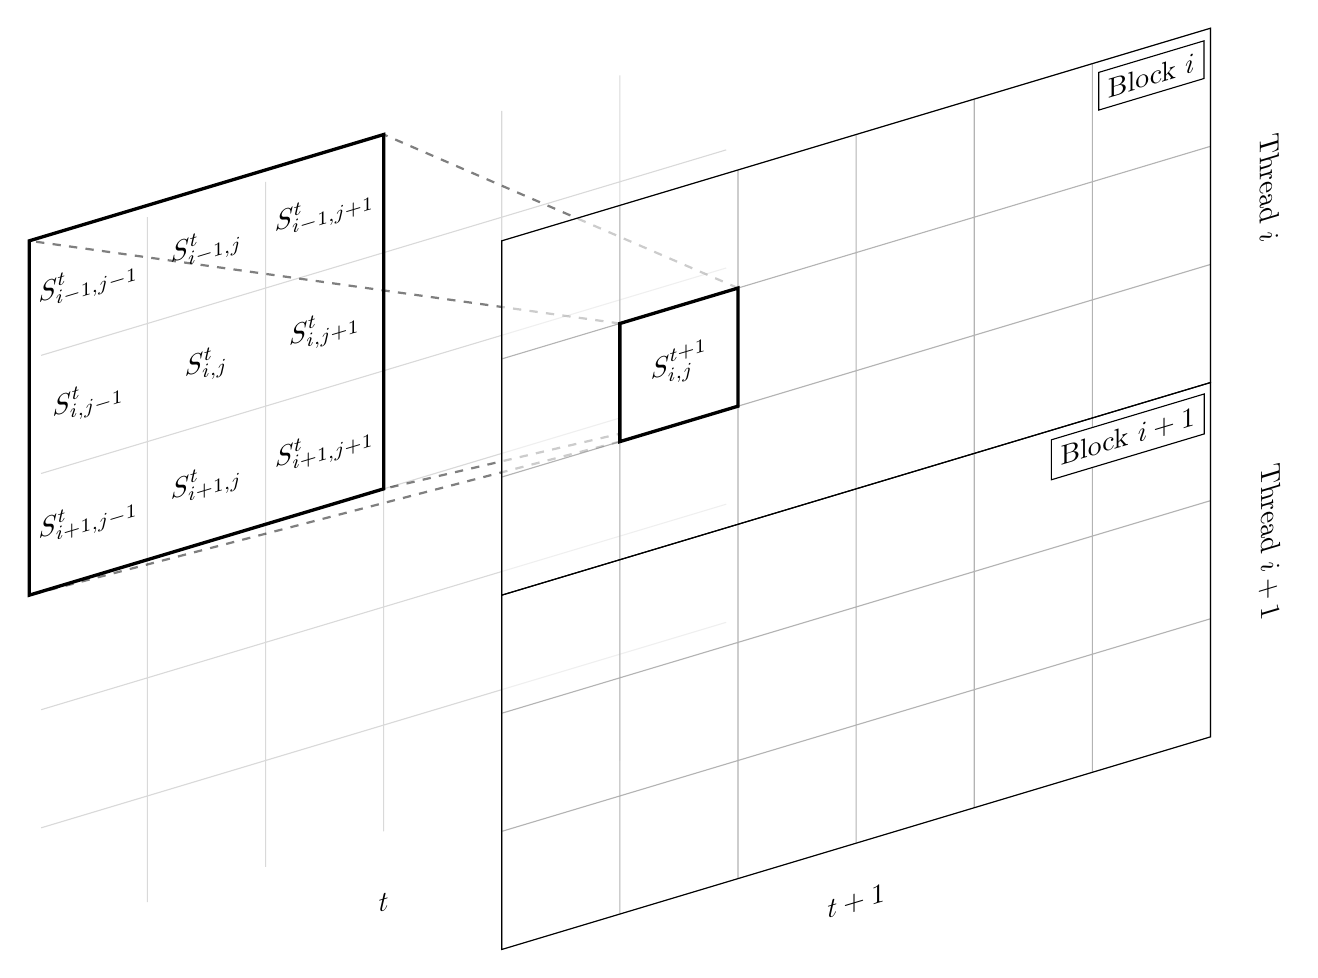
\begin{tikzpicture}[scale=1.5]

     \begin{scope}[every node/.append style={yslant=0.3},yslant=0.3]
        \draw[gray, opacity=0.3] (0.1, 0.1) grid (5.9, 5.9);
        \draw[very thick] (0, 6) -- (3, 6) --  (3, 3) -- (0, 3) -- cycle;
        %\draw[ultra thick] (-1, 3) -- (7,3);
        \node[anchor=center] at (1.5, 4.5) {$S_{i,j}^t$};
        \node[anchor=center] at (1.5, 5.5) {$S_{i-1,j}^t$};
        \node[anchor=center] at (1.5, 3.5) {$S_{i+1,j}^t$};
        \node[anchor=center] at (0.5, 4.5) {$S_{i,j-1}^t$};
        \node[anchor=center] at (2.5, 4.5) {$S_{i,j+1}^t$};
        \node[anchor=center] at (0.5, 5.5) {$S_{i-1,j-1}^t$};
        \node[anchor=center] at (0.5, 3.5) {$S_{i+1,j-1}^t$};
        \node[anchor=center] at (2.5, 5.5) {$S_{i-1,j+1}^t$};
        \node[anchor=center] at (2.5, 3.5) {$S_{i+1,j+1}^t$};
        \node[anchor=center] at (3, -0.5) {$t$};
    \end{scope}
    
    \begin{scope}[xshift=4cm,every node/.append style={yslant=0.3},yslant=0.3]
        \draw[dashed, thick, opacity=0.5] (1, 5) -- (-4, 7.2);
        \draw[dashed, thick, opacity=0.5] (1, 4) -- (-4, 4.2);
        \draw[dashed, thick, opacity=0.5] (2, 5) -- (-1, 7.2);
        \draw[dashed, thick, opacity=0.5] (2, 4) -- (-1, 4.2);
        \draw[draw=gray, fill=white, opacity=0.6] (0, 0) grid (6, 6) rectangle (0, 0);
        \draw[very thick, fill=white] (1, 5) -- (2, 5) --  (2, 4) -- (1, 4) -- cycle;
        
        %\draw[ultra thick] (-1, 3) -- (7,3);
        \node[anchor=center] at (1.5, 4.5) {$S_{i,j}^{t+1}$};
        
        \draw (0,3) rectangle (6,6);
        \draw (0,0) rectangle (6,3);
        
        %\draw[dash dot, ultra thick] (-1, 3) -- (7, 3);
        \node[anchor=center] at (3, -0.5) {$t+1$};
        \node[draw, fill=white] at (5.5, 5.75) {Block $i$};
        \node[draw, fill=white] at (5.3, 2.75) {Block $i+1$};
        \node [rotate=-90] at (6.5, 4.5) {Thread $i$};
        \node [rotate=-90] at (6.5, 1.5) {Thread $i+1$};
    \end{scope}
    
\end{tikzpicture}
            }    
            \caption{\emph{SubSpreading} computing a matrix block.}
            \label{fig:thread}
        \end{figure}
        
        
\section{Evaluation}
    
    In this section we present some simulations to compare the performance of our proposal model.
    We assume the use of a square grid of size $N \times N$ and, defining the maximum number
    of discrete times $T_{max}$ we estimate a computational complexity of $O(T_{max}\cdot N^2)$. 
    
    It is important to mention that in the case we choose $T_{max} << N$ the complexity is about $O(N^2)$,
    but it may change a lot if $T_{max}\sim N$ increasing the complexity to $O(N^3)$. This is the main 
    motivation of to include the use of threads in the computing of the model.
    
    The experiments were made using a fixed $T_{max}=50$, for $1$ to $4$ number of threads, repeating the 
    simulations $10$ times per $N$. The average of these repetitions are summarized in Table~\ref{tab:results}.
    
    \begin{table}[!ht]
        \renewcommand{\arraystretch}{1.3}
        \centering
        \caption{Summary of the average times in seconds.}
        \label{tab:results}
        \begin{tabular}{c||rrrr}
            \hline
            Threads & $N=100$ & $N=500$ & $N=1000$ & $N=1500$ \\ \hline\hline
            1       & $0.198$   & $8.023$   & $32.861$   & $72.464$   \\
            2       & $0.135$   & $5.147$   & $19.695$   & $44.407$   \\
            3       & $0.163$   & $4.825$   & $18.852$   & $41.626$   \\
            4       & $0.220$   & $4.650$   & $18.055$   & $41.458$  
        \end{tabular}
    \end{table}

    To show a better representation of results and compare to the theoretical complexity estimated, we 
    present the Figure~\ref{fig:benchmark}.
    
    \begin{figure}[!ht]
        \centering
        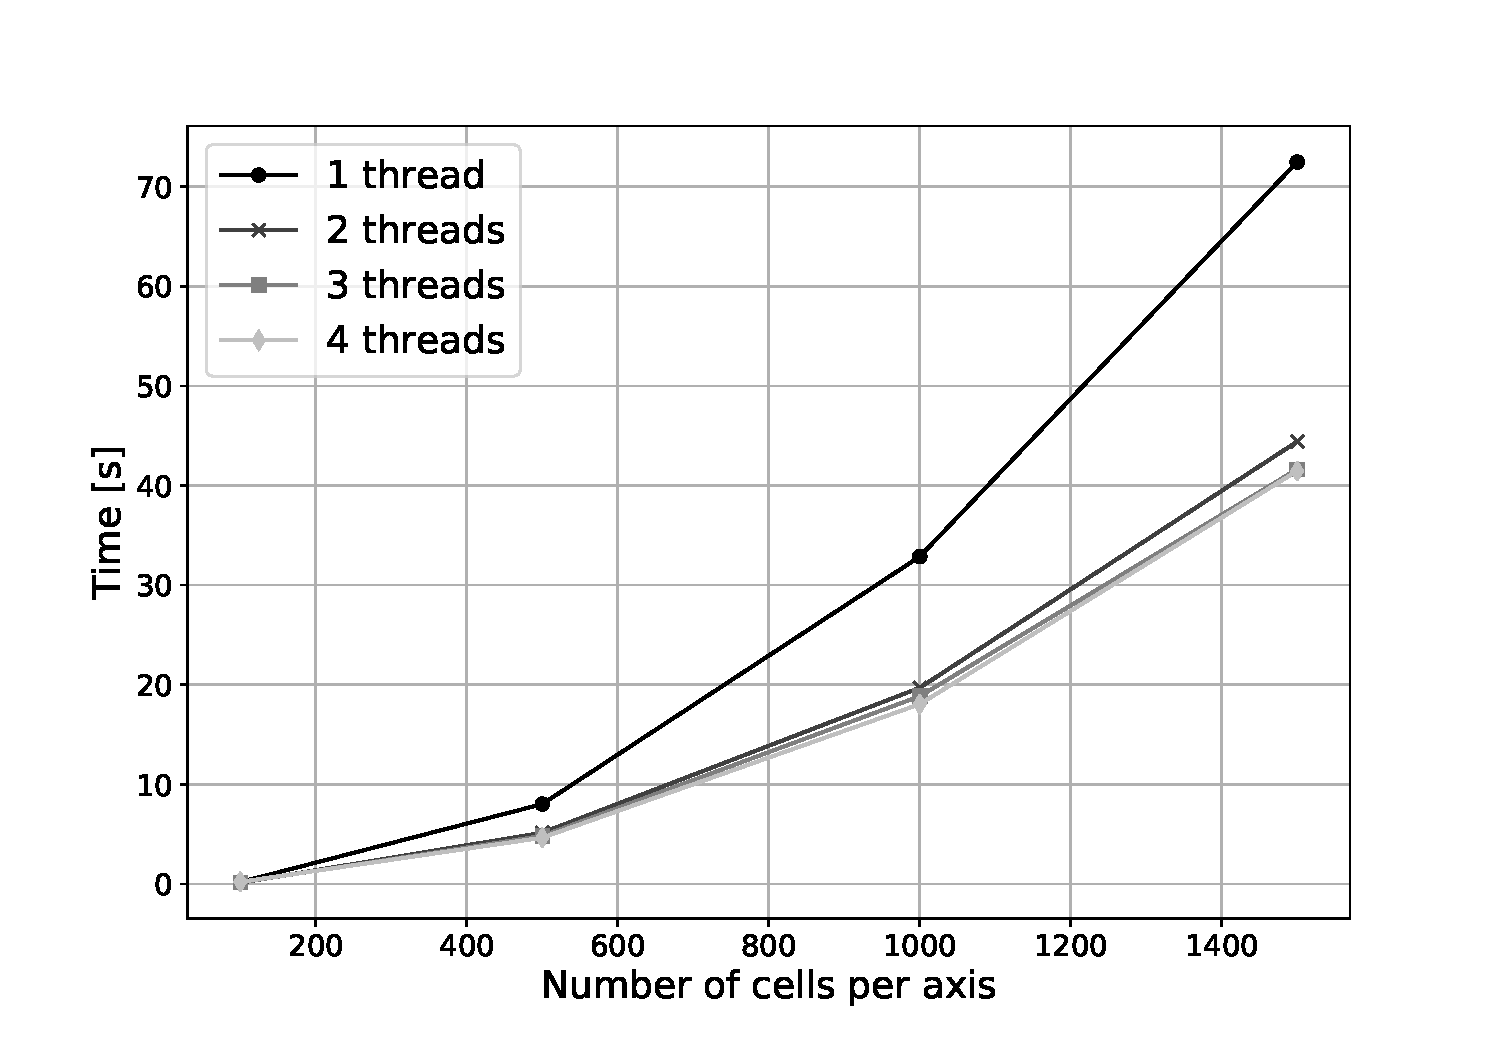
\includegraphics[width=3in,height=3in,clip,keepaspectratio]{img/benchmark.pdf}
        \caption{Threads' performance comparison}
        \label{fig:benchmark}
    \end{figure}
    
    We note that the curves approximate the estimated complexity. In addition we can appreciate the impact of 
    the parallel implementation in the computation time of the simulations. Computing the Speedup $S$ as
    \begin{equation}
        S = \frac{Time_{sequential}}{Time_{parallel}},
    \end{equation}
    
    we resume the \emph{Speedup} results in Table~\ref{tab:speedups}.
    
    \begin{table}[!ht]
        \renewcommand{\arraystretch}{1.3}
        \centering
        \caption{Speedups results.}
        \label{tab:speedups}
        \begin{tabular}{c||rrrr}
            \hline
            Threads & $N=100$ & $N=500$ & $N=1000$ & $N=1500$ \\ \hline\hline
            2       & $1.47$ & $1.56$ & $1.67$ & $1.63$ \\
            3       & $1.21$ & $1.66$ & $1.74$ & $1.74$ \\
            4       & $0.90$ & $1.73$ & $1.82$ & $1.75$  
        \end{tabular}
    \end{table}
    
    
    For a qualitative evaluation Figure~\ref{fig:simulation} shows a piece of map simulated for 
    $N=1500$, $T=30^{\circ}$C, $H=50$\%, $W_s=40$ km/hr, $W_d=90^{\circ}$, $P=50$ hPa, 
    $F_{23} = F_{24}= F_{42} = 0.1$.
    
    \begin{figure}[!ht]
        \centering
        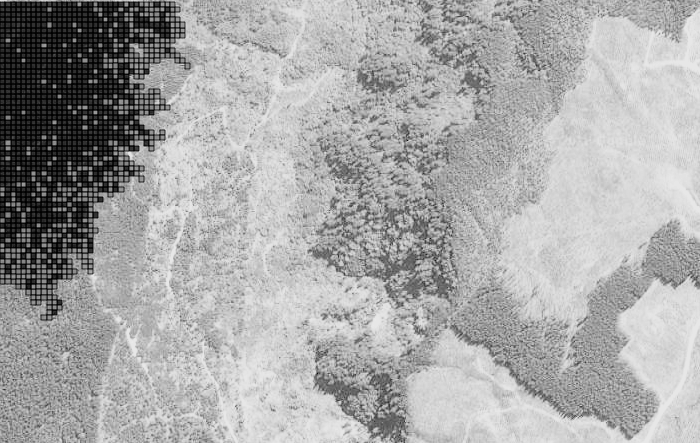
\includegraphics[width=3in,height=3in,clip,keepaspectratio]{img/simulation_gray.png}
        \caption{Simulation's qualitative result.}
        \label{fig:simulation}
    \end{figure}
    

\section{Validation/Discussion}
    
    According to \cite{preisler2013forest} fire models can be grouped into three types: risk models, 
    propagation and effect. The first ones are associated to quantify the probability and potential effects before
    possible episodes of fire. Depending on the variables used, different jobs can be found, for example
    the estimation of the probability of occurrence of a fire depending on the location and the day of the year
    \cite{brillinger2003risk, hernandez2010integrating}, fire hazard and climate indices \cite{van1987development,
    burgan19881988}, among others \cite{braun2010forest, ager2007modeling, calkin2011comparative}. The second group tries
    model the movement of fire and exist from physical approaches \cite{rothermel1972mathematical} to models of
    regression to estimate the propagation rate \cite{sullivan2009wildland}. Generally this type of models assumes that
    the fuel (place where the fire occurs) can be tiled by a regular mesh where each cell has
    associated a probability of burning and that depends on the conditions of the neighboring cells. There are different
    tools associated with this type of models and can be reviewed in \cite{andrews1986behave, finney2006overview,
    finney1998farsite, finney2011simulation, finney2011method}. Finally, the effect models are important
    to study the administration and management of fuels, for example the control of tree mortality
    or analysis of ecosystems, among others \cite{Larkin-2009, reinhardt2003using, robichaud2007predicting}. \medskip
    
    As mentioned in the introduction, modeling with differential equations is one of the most used approaches. 
    The main problem with wildfire models based on this approach is the computational cost associated with the 
    resolution of the equations. For example, the reaction-convection-diffusion equation \cite{liu2009elementary} is 
    a mathematical model that models temperature and involves the effect of a flow and the reaction rate of 
    chemicals interpreted as fuel. One of the most used numerical methods to solve diffusion equations is the 
    Crank-Nicolson method, which is known to have computational cost problems when solving the problem in two 
    dimensions, given the size of the system of equations that is required to solve for each iteration in time. 
    In addition, the flow or wind, which is represented by a vector field, must satisfy the Navier-Stokes 
    equations, a problem that does not have a general solution \cite{fefferman2006existence}, so it can usually 
    only be approximated with a high computational cost. The dynamic implementation is a problem for differential
    equations since the increment of complexity unlike the model proposed by us for example in the modification
    of environmental conditions that only implies to set values in the matrices of the discrete world. \medskip
    
    The wildfire dynamics generated with the prototypes are consistent with what CONAF has observed in past 
    devastating wildfires occurring in Chile. Nevertheless, the effort so far has focused in creating a 
    framework to include the core of modelling found in related work and mainly the expert’s knowledge and 
    expertise through manipulation of quantitative and qualitative variables affecting the dynamics.  

    Dynamic interplay among temperature, pressure, and humidity is a key element to be included in models for 
    wildfire in Chilean context. While this has been approach from a qualitative decision making perspective 
    in this version of the model, more elaborate local level rules for the interplay among these variables will 
    be explore in a future version of the wildfire dynamics model. 

\section{Conclusion}
    
    This article describes a qualitative approach to calibrate and generate a suitable model for realistic 
    wildfire dynamics for three high priority protection rural location for the Chilean forest fire agency. 
    This modelling effort is based on discrete simulation using a Cellular Automata to simulate fire spreading, 
    which is easy to manipulate at both quantitative low level and qualitative high level. As expected, the system’s 
    dynamics emerging from cell’s switching rules involving environmental, topographic, and fuel components, as well 
    as experts’ suggested features, such as smoke column characteristics, facilitates the use of an expert-based try 
    and error approach to achieve suitable and realistic wildfire dynamics. 
    
    The incorporation of parallel techniques allows the model to compute enough states in discrete times to show 
    a qualitatively realistic result for the specialists' requirements. The decrease in computing time allows 
    us to conclude that the use of multithreads is a good strategy to apply to this problem, given the characteristics 
    of the discrete world and the independence of states between the times $t$ and $t + 1$.

    On the other hand, the incorporation of experts into the development, calibration, and evaluation of the wildfire 
    dynamics model being built became a key component in achieving models that resemble the dynamics of devastating 
    wildfires occurring in the locations modeled in this work. The provision of all the parameters governing the 
    dynamics of the wildfire in the prototypes built allowed the experts to use their expertise and knowledge to 
    manipulate those parameters to gradually achieve suitable and realistic outcomes. 

    Finally, positive qualitative evaluation has been obtained from wildfire combat experts, from the Chilean forest 
    fire agency in terms of functionality, usability, performance, and overall quality of the prototypes built upon the 
    wildfire model designed in this research effort. These experts also highlighted that the introduction of the 
    expert to be able to change at will the conditions and ongoing wildfire dynamics is of extreme value to provide 
    not only suitable and realistic simulations, but also for increasing the learning experience on professionals who
    would be using the simulator, from which the model presented in this article is part of.
    
    
\section{Future Work}
    
    Future work will seek to deliver more solid components, or finer granularity in some cases, for the core 
    characteristics of the wildfire dynamics, such as the topographic and fuel components. \medskip
    
    Another possibility of improvement is related to the use of a parallel architecture of the pipeline type, 
    taking advantage of the refresh rate in the interface of the simulator. It is evident that in addition to 
    the efforts in the speed of computation we must include work in the optimization of communication and memory usage.

% if have a single appendix:
%\appendix[Proof of the Zonklar Equations]
% or
%\appendix  % for no appendix heading
% do not use \section anymore after \appendix, only \section*
% is possibly needed

% use appendices with more than one appendix
% then use \section to start each appendix
% you must declare a \section before using any
% \subsection or using \label (\appendices by itself
% starts a section numbered zero.)
%


%\appendices
%\section{Proof of the First Zonklar Equation}
%\blindtext

% use section* for acknowledgement
%\section*{Acknowledgment}

%The authors would like to thank...


% Can use something like this to put references on a page
% by themselves when using endfloat and the captionsoff option.
\ifCLASSOPTIONcaptionsoff
  \newpage
\fi



% trigger a \newpage just before the given reference
% number - used to balance the columns on the last page
% adjust value as needed - may need to be readjusted if
% the document is modified later
%\IEEEtriggeratref{8}
% The "triggered" command can be changed if desired:
%\IEEEtriggercmd{\enlargethispage{-5in}}

% references section

% can use a bibliography generated by BibTeX as a .bbl file
% BibTeX documentation can be easily obtained at:
% http://www.ctan.org/tex-archive/biblio/bibtex/contrib/doc/
% The IEEEtran BibTeX style support page is at:
% http://www.michaelshell.org/tex/ieeetran/bibtex/
\bibliographystyle{IEEEtran}
\bibliography{IEEEabrv,IEEEreferences}
% argument is your BibTeX string definitions and bibliography database(s)
%\bibliography{IEEEabrv,../bib/paper}
%
% <OR> manually copy in the resultant .bbl file
% set second argument of \begin to the number of references
% (used to reserve space for the reference number labels box)
% \begin{thebibliography}{1}

% \bibitem{IEEEhowto:kopka}
% H.~Kopka and P.~W. Daly, \emph{A Guide to \LaTeX}, 3rd~ed.\hskip 1em plus
%   0.5em minus 0.4em\relax Harlow, England: Addison-Wesley, 1999.

% \end{thebibliography}

% biography section
% 
% If you have an EPS/PDF photo (graphicx package needed) extra braces are
% needed around the contents of the optional argument to biography to prevent
% the LaTeX parser from getting confused when it sees the complicated
% \includegraphics command within an optional argument. (You could create
% your own custom macro containing the \includegraphics command to make things
% simpler here.)
%\begin{biography}[{\includegraphics[width=1in,height=1.25in,clip,keepaspectratio]{mshell}}]{Michael Shell}
% or if you just want to reserve a space for a photo:

\begin{IEEEbiography}[{\includegraphics[width=1in,height=1.25in,clip,keepaspectratio]{picture}}]{John Doe}
%\blindtext
\end{IEEEbiography}

% You can push biographies down or up by placing
% a \vfill before or after them. The appropriate
% use of \vfill depends on what kind of text is
% on the last page and whether or not the columns
% are being equalized.

%\vfill

% Can be used to pull up biographies so that the bottom of the last one
% is flush with the other column.
%\enlargethispage{-5in}




% that's all folks
\end{document}


